\documentclass{beamer}

% === AUTOR === (((
\author{\textit{Por Erick I. Rodríguez Juárez.}}
% )))

% === PAQUETES === (((
% \usepackage{makeidx}
% \usepackage{xltxtra}
\usepackage{amsfonts}
\usepackage{amsmath}
\usepackage{amssymb}
% \usepackage{fullpage}
\usepackage{tikz}
\usetikzlibrary{arrows.meta}
\usepackage{graphicx}
% )))

% === TIPOGRAFÍA === (((
% \setmainfont[
  % BoldFont       = bodonibi,
	% ItalicFont     = Century modern italic2.ttf,
	% BoldItalicFont = bodonibi,
	% SmallCapsFont  = lmromancaps10-regular.otf
% ]{Century_modern.ttf}
% )))

% === COMANDOS === (((
% \newcommand{\dis}{\displaystyle}
% \newcommand{\qed}{\hspace{0.5cm}\rule{0.16cm}{0.4cm}}
% \newcommand{\operator}[1]{\mathop{\vphantom{\sum}\mathchoice
% {\vcenter{\hbox{\huge $#1$}}}
% {\vcenter{\hbox{\Large $#1$}}}{#1}{#1}}\displaylimits}
% \newcommand{\suma}{\operator{
\includegraphics[scale=0.09]{FOTOS/Sigma.png}}}
% \setlength{\parindent}{0mm}
% )))

% === ITALICA EN ENTORNO MATEMÁTICO === (((
% \DeclareSymbolFont{italics}{\encodingdefault}{\rmdefault}{m}{it}
% \DeclareSymbolFontAlphabet{\mathit}{italics}
% \ExplSyntaxOn
% \int_step_inline:nnnn { `A } { 1 } { `Z }
 % {  \exp_args:Nf \DeclareMathSymbol{\char_generate:nn{#1}{11}}{\mathalpha}{italics}{#1} }
% \int_step_inline:nnnn { `a } { 1 } { `z } {  \exp_args:Nf \DeclareMathSymbol{\char_generate:nn{#1}{11}}{\mathalpha}{italics}{#1}}
% \ExplSyntaxOff
% )))

\begin{document}

\frame{\titlepage}

\begin{frame}[t]
	\frametitle{Teorema de Existencia y Unicidad.}
\begin{block}{Teorema de Existencia y Unicidad.}
	Considere el P.V.I. siguiente
	\[
		a_n(x) y^{(n)} + a_{n-1} (x) y^{(n-1)} + \;\cdots\; + a_1(x) y' +a_0(x) y = g(x).
	\]
	Sujeto a \(a_n(x) , a_{n-1} (x) , \;\cdots\; a_1(x) ,a_0(x)\) y \(g(x)\) continuas en el intervalo \(I\) y además, \(a_n(x) \ne 0\), \(\forall x \in I\). Si \(x=x_0\) en cualquier punto en el intervalo \(I\), entonces existe una única solución para el P.V.I. en \(I\).
\end{block}
	\begin{example}
		Determina si el P.V.I. \(x^2y'' -2xy' +2y=6\), \(y(0) =3\), \(y' (0) =1\), para \(x \in (- \infty , \infty)\) tiene solución única usando e T.E. y U.
	\end{example}
\end{frame}
\begin{frame}[t]
\end{frame}

\begin{frame}[t]
	\begin{minipage}{0.6\linewidth}
		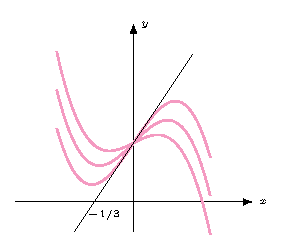
\includegraphics[width= \linewidth]{IMAGENES/6/tikz.pdf}
	\end{minipage}
	\begin{minipage}{0.3\linewidth}
	\end{minipage}
\end{frame}

\begin{frame}[t]
	\begin{example}
		Considere la siguiente E.D. \(x'' +16x=0\), y \(x(t) = c_1 \cos 4t+c_2 \sin 4t\), la solución general explícita de dicha E.D. Entonces la solución del problema en la frontera cuyas condiciones son:
		\begin{enumerate}
			\item \(x(0) =0\), \(x(\pi /2) =0\).
			\item \(x(0) =0\), \(x(\pi /2) =1\).
			\item \(x(0) =0\), \(x(\pi /8) =0\).
		\end{enumerate}
	\end{example}
\end{frame}

\end{document}
